\documentclass{standalone}
%
\usepackage{tikz}
\usetikzlibrary{backgrounds,calc}
\usepackage{tkz-euclide}
\usetkzobj{all}
%
\usepackage{amsmath}
%
\usepackage{xcolor}
%
\definecolor{space}{HTML}{0A2543}
\definecolor{earth}{HTML}{0089FA}
\definecolor{mars}{HTML}{DC7B4E}
%
\title{Trigonometry: ArcTan pi/4}
\begin{document}
	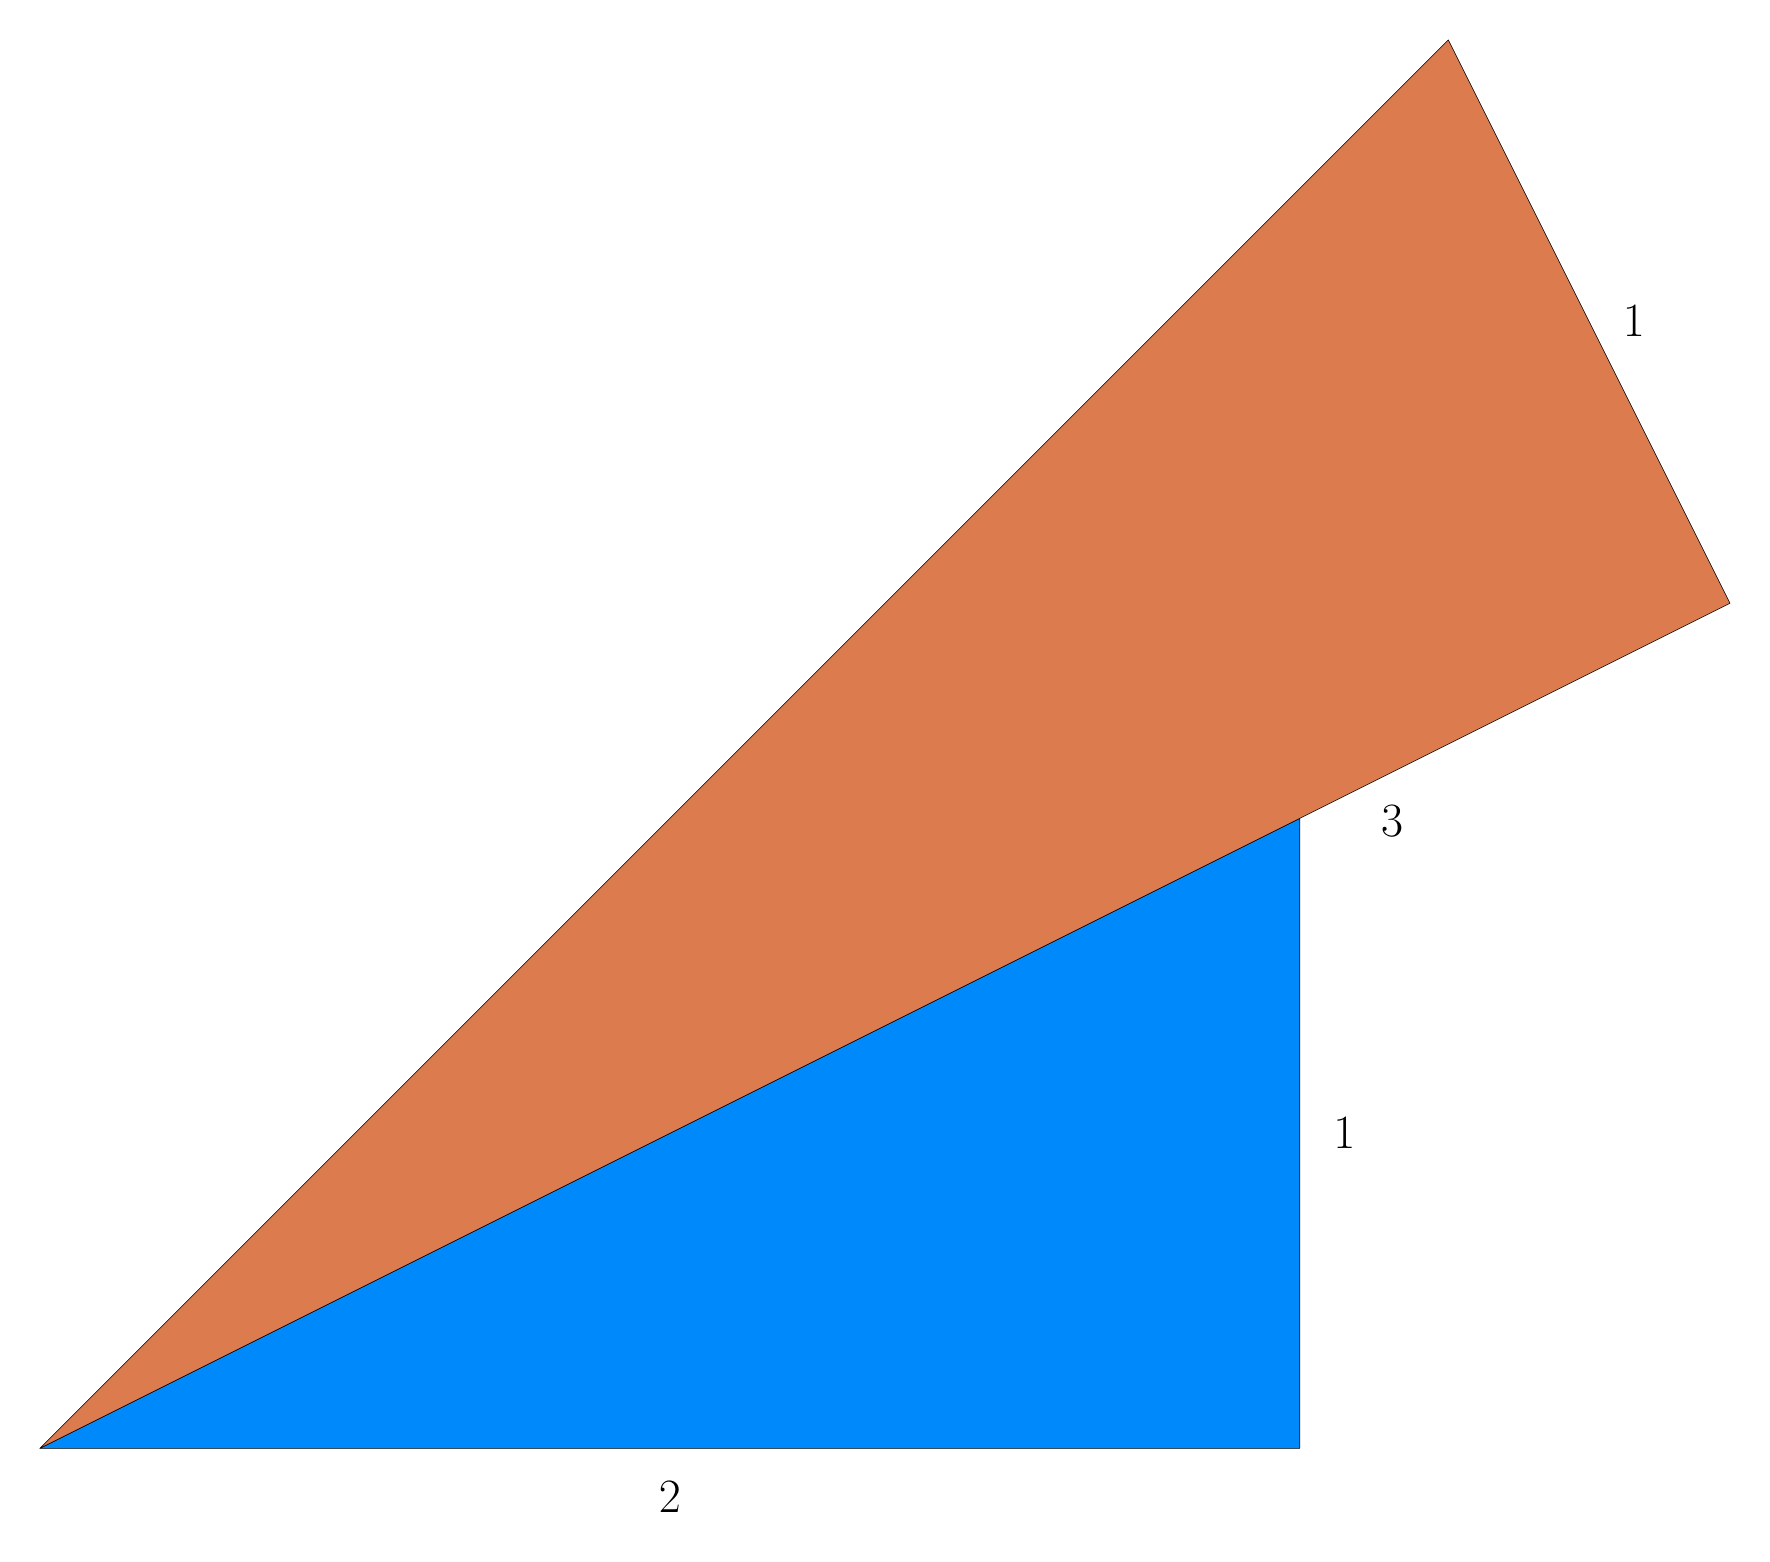
\begin{tikzpicture}[background rectangle/.style={fill=white},show background rectangle]
	%
	\begin{scope}[scale=8]
		\tkzDefPoint(0,0){O}
		\tkzDefPoint(2,0){A}
		\tkzDefPoint(2,1){B}
		\tkzDrawSquare[fill=space](O,A)
		%
		\tkzDrawPolygon[fill=earth](O,A,B)
		%
		\tkzDefPoint(3,0){C}
		\tkzDefPoint(3,1){D}
		\tkzDefPointBy[rotation = center O angle {atan(1/2)}](C) \tkzGetPoint{C1}
		\tkzDefPointBy[rotation = center O angle {atan(1/2)}](D) \tkzGetPoint{D1}
		%
		\tkzDrawPolygon[fill=mars](O,C1,D1)
		%
		\tkzLabelSegment[black,below=2ex,pos=.5](O,A){\fontsize{17}{18}\selectfont $2$}
		\tkzLabelSegment[black,right=2ex,pos=.5](A,B){\fontsize{17}{18}\selectfont $1$}
		\tkzLabelSegment[black,below=2ex,pos=0.8](O,C1){\fontsize{17}{18}\selectfont $3$}
		\tkzLabelSegment[black,right=2ex,pos=.5](C1,D1){\fontsize{17}{18}\selectfont $1$}
		%
		\node at (0.5,1.5) {\textcolor{white}{\fontsize{17}{18}\selectfont $\arctan \frac{1}{2} + \arctan \frac{1}{3} = \frac{\pi}{4}$}};
	\end{scope}
	%
	\end{tikzpicture}
\end{document}